\documentclass[tikz,border=10pt]{standalone}
\usepackage{amsmath}
\usepackage{tikz}
\usetikzlibrary{shapes,arrows,positioning,calc,decorations.pathreplacing}

% Tensor network styles
\tikzset{
    tensor/.style={draw, fill=blue!20, minimum size=0.8cm, rounded corners=2pt},
    tensorU/.style={draw, fill=green!20, minimum size=0.8cm, rounded corners=2pt},
    tensorS/.style={draw, fill=yellow!30, minimum size=0.6cm, circle},
    tensorV/.style={draw, fill=red!20, minimum size=0.8cm, rounded corners=2pt},
    tensorA/.style={draw, fill=green!30, minimum size=0.7cm, rounded corners=2pt},
    tensorRem/.style={draw, fill=orange!20, minimum size=0.8cm, rounded corners=2pt},
    iso/.style={draw, fill=green!30, isosceles triangle, isosceles triangle apex angle=60,
                minimum width=0.8cm, minimum height=0.7cm, inner sep=1pt},
    bond/.style={thick},
    ext/.style={thick},
    label/.style={font=\small},
    equals/.style={font=\Large},
}

\begin{document}

% ============================================
% Diagram 1: Full tensor and initial reshape
% ============================================
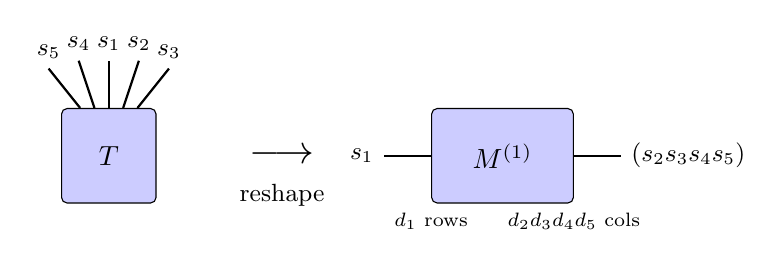
\begin{tikzpicture}[scale=1]
    % Full tensor
    \node[tensor, minimum size=1.2cm] (T) at (0,0) {$T$};

    % External indices
    \draw[ext] (T.north) -- ++(0,0.6) node[above, label] {$s_1$};
    \draw[ext] ($(T.north)!0.3!(T.north east)$) -- ++(0.2,0.6) node[above, label] {$s_2$};
    \draw[ext] ($(T.north)!0.6!(T.north east)$) -- ++(0.4,0.5) node[above, label] {$s_3$};
    \draw[ext] ($(T.north)!0.3!(T.north west)$) -- ++(-0.2,0.6) node[above, label] {$s_4$};
    \draw[ext] ($(T.north)!0.6!(T.north west)$) -- ++(-0.4,0.5) node[above, label] {$s_5$};

    % Arrow
    \node[equals] at (2.2,0) {$\longrightarrow$};
    \node[font=\small] at (2.2,-0.5) {reshape};

    % Matrix form
    \node[tensor, minimum width=1.8cm, minimum height=1.2cm] (M) at (5,0) {$M^{(1)}$};

    % Matrix indices
    \draw[ext] (M.west) -- ++(-0.6,0) node[left, label] {$s_1$};
    \draw[ext] (M.east) -- ++(0.6,0) node[right, label] {$(s_2 s_3 s_4 s_5)$};

    % Dimension labels
    \node[font=\scriptsize, below] at (M.south west) {$d_1$ rows};
    \node[font=\scriptsize, below] at (M.south east) {$d_2 d_3 d_4 d_5$ cols};
\end{tikzpicture}

% ============================================
% Diagram 2: SVD decomposition step
% ============================================
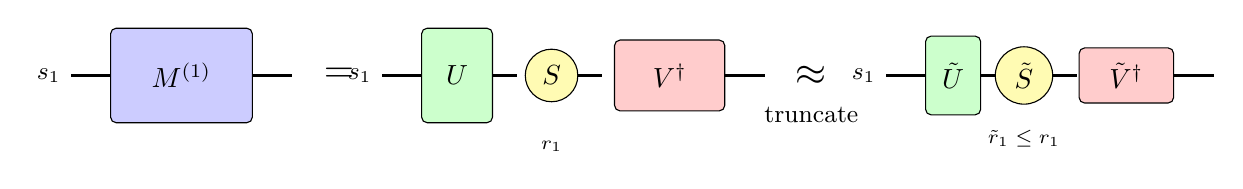
\begin{tikzpicture}[scale=1]
    % Matrix
    \node[tensor, minimum width=1.8cm, minimum height=1.2cm] (M) at (0,0) {$M^{(1)}$};
    \draw[ext] (M.west) -- ++(-0.5,0) node[left, label] {$s_1$};
    \draw[ext] (M.east) -- ++(0.5,0);

    % Equals
    \node[equals] at (2,0) {$=$};

    % U matrix
    \node[tensorU, minimum width=0.9cm, minimum height=1.2cm] (U) at (3.5,0) {$U$};
    \draw[ext] (U.west) -- ++(-0.5,0) node[left, label] {$s_1$};
    \draw[bond] (U.east) -- ++(0.3,0);

    % S matrix (diagonal)
    \node[tensorS] (S) at (4.7,0) {$S$};
    \draw[bond] (S.east) -- ++(0.3,0);

    % V^dagger matrix
    \node[tensorV, minimum width=1.4cm, minimum height=0.9cm] (V) at (6.2,0) {$V^\dagger$};
    \draw[ext] (V.east) -- ++(0.5,0);

    % Bond dimension label
    \node[font=\scriptsize] at (4.7, -0.9) {$r_1$};

    % Arrow to truncated version
    \node[equals] at (8,0) {$\approx$};
    \node[font=\small] at (8,-0.5) {truncate};

    % Truncated U
    \node[tensorU, minimum width=0.7cm, minimum height=1.0cm] (Ut) at (9.8,0) {$\tilde{U}$};
    \draw[ext] (Ut.west) -- ++(-0.5,0) node[left, label] {$s_1$};
    \draw[bond] (Ut.east) -- ++(0.3,0);

    % Truncated S
    \node[tensorS, minimum size=0.5cm] (St) at (10.7,0) {$\tilde{S}$};
    \draw[bond] (St.east) -- ++(0.3,0);

    % Truncated V^dagger
    \node[tensorV, minimum width=1.2cm, minimum height=0.7cm] (Vt) at (12,0) {$\tilde{V}^\dagger$};
    \draw[ext] (Vt.east) -- ++(0.5,0);

    % Truncated bond dimension
    \node[font=\scriptsize] at (10.7, -0.8) {$\tilde{r}_1 \leq r_1$};
\end{tikzpicture}

% ============================================
% Diagram 3: First tensor extracted
% ============================================
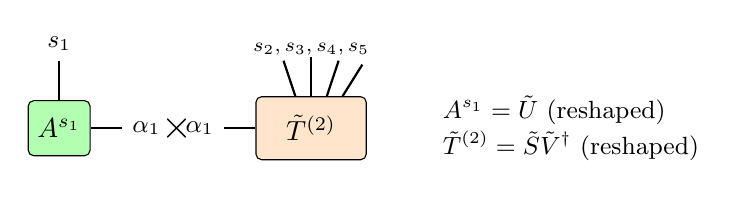
\begin{tikzpicture}[scale=1]
    % Truncated U becomes A^{s_1}
    \node[tensorA] (A1) at (0,0) {$A^{s_1}$};
    \draw[ext] (A1.north) -- ++(0,0.5) node[above, label] {$s_1$};
    \draw[bond] (A1.east) -- ++(0.4,0) node[right, label] {$\alpha_1$};

    % Multiplication sign
    \node[font=\Large] at (1.5,0) {$\times$};

    % Remainder tensor
    \node[tensorRem, minimum width=1.4cm] (R) at (3.2,0) {$\tilde{T}^{(2)}$};
    \draw[bond] (R.west) -- ++(-0.4,0) node[left, label] {$\alpha_1$};
    \draw[ext] (R.north) -- ++(0,0.5);
    \draw[ext] ($(R.north)+(0.2,0)$) -- ++(0.15,0.45);
    \draw[ext] ($(R.north)+(-0.2,0)$) -- ++(-0.15,0.45);
    \draw[ext] ($(R.north)+(0.4,0)$) -- ++(0.25,0.4);
    \node[font=\scriptsize] at (3.2, 1.0) {$s_2, s_3, s_4, s_5$};

    % Explanation
    \node[font=\small, align=left] at (6.5, 0) {$A^{s_1} = \tilde{U}$ (reshaped)\\[2pt]
    $\tilde{T}^{(2)} = \tilde{S}\tilde{V}^\dagger$ (reshaped)};
\end{tikzpicture}

% ============================================
% Diagram 4: Full TT-SVD iteration process
% ============================================
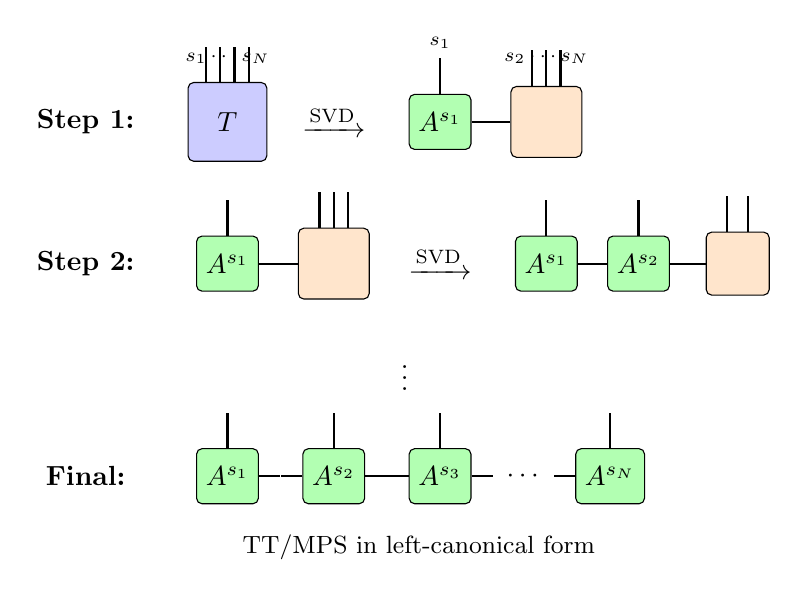
\begin{tikzpicture}[scale=0.9]
    % Step 1: Full tensor
    \node[font=\bfseries] at (-2, 0) {Step 1:};
    \node[tensor, minimum size=1cm] (T1) at (0,0) {$T$};
    \foreach \i/\x in {1/-0.3, 2/-0.1, 3/0.1, 4/0.3} {
        \draw[ext] ($(T1.north)+(\x,0)$) -- ++(0,0.5);
    }
    \node[font=\scriptsize] at (0, 0.9) {$s_1 \cdots s_N$};

    \node at (1.5,0) {$\xrightarrow{\text{SVD}}$};

    % After first SVD
    \node[tensorA] (A1) at (3,0) {$A^{s_1}$};
    \draw[ext] (A1.north) -- ++(0,0.5) node[above, font=\scriptsize] {$s_1$};
    \draw[bond] (A1.east) -- ++(0.3,0);

    \node[tensorRem, minimum size=0.9cm] (R1) at (4.5,0) {};
    \draw[bond] (R1.west) -- ++(-0.3,0);
    \foreach \i/\x in {1/-0.2, 2/0, 3/0.2} {
        \draw[ext] ($(R1.north)+(\x,0)$) -- ++(0,0.5);
    }
    \node[font=\scriptsize] at (4.5, 0.9) {$s_2 \cdots s_N$};

    % Step 2
    \node[font=\bfseries] at (-2, -2) {Step 2:};
    \node[tensorA] (A1b) at (0,-2) {$A^{s_1}$};
    \draw[ext] (A1b.north) -- ++(0,0.5);
    \draw[bond] (A1b.east) -- ++(0.3,0);

    \node[tensorRem, minimum size=0.9cm] (R1b) at (1.5,-2) {};
    \draw[bond] (R1b.west) -- ++(-0.3,0);
    \foreach \i/\x in {1/-0.2, 2/0, 3/0.2} {
        \draw[ext] ($(R1b.north)+(\x,0)$) -- ++(0,0.5);
    }

    \node at (3,-2) {$\xrightarrow{\text{SVD}}$};

    \node[tensorA] (A1c) at (4.5,-2) {$A^{s_1}$};
    \draw[ext] (A1c.north) -- ++(0,0.5);
    \draw[bond] (A1c.east) -- ++(0.3,0);

    \node[tensorA] (A2c) at (5.8,-2) {$A^{s_2}$};
    \draw[bond] (A2c.west) -- ++(-0.3,0);
    \draw[ext] (A2c.north) -- ++(0,0.5);
    \draw[bond] (A2c.east) -- ++(0.3,0);

    \node[tensorRem, minimum size=0.8cm] (R2c) at (7.2,-2) {};
    \draw[bond] (R2c.west) -- ++(-0.3,0);
    \foreach \i/\x in {1/-0.15, 2/0.15} {
        \draw[ext] ($(R2c.north)+(\x,0)$) -- ++(0,0.5);
    }

    % Dots
    \node at (2.5, -3.5) {$\vdots$};

    % Final step
    \node[font=\bfseries] at (-2, -5) {Final:};

    \node[tensorA] (Af1) at (0,-5) {$A^{s_1}$};
    \draw[ext] (Af1.north) -- ++(0,0.5);
    \draw[bond] (Af1.east) -- ++(0.3,0);

    \node[tensorA] (Af2) at (1.5,-5) {$A^{s_2}$};
    \draw[bond] (Af2.west) -- ++(-0.3,0);
    \draw[ext] (Af2.north) -- ++(0,0.5);
    \draw[bond] (Af2.east) -- ++(0.3,0);

    \node[tensorA] (Af3) at (3,-5) {$A^{s_3}$};
    \draw[bond] (Af3.west) -- ++(-0.3,0);
    \draw[ext] (Af3.north) -- ++(0,0.5);
    \draw[bond] (Af3.east) -- ++(0.3,0);

    \node at (4.2, -5) {$\cdots$};

    \node[tensorA] (AfN) at (5.4,-5) {$A^{s_N}$};
    \draw[bond] (AfN.west) -- ++(-0.3,0);
    \draw[ext] (AfN.north) -- ++(0,0.5);

    % Label
    \node[font=\small] at (2.7, -6) {TT/MPS in left-canonical form};
\end{tikzpicture}

% ============================================
% Diagram 5: Left-canonical property
% ============================================
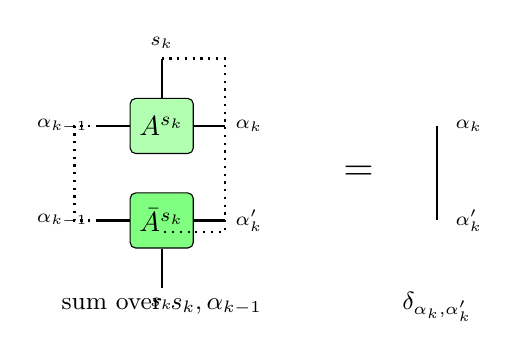
\begin{tikzpicture}[scale=1]
    % Left orthogonality condition
    \node[tensorA] (A) at (0,0) {$A^{s_k}$};
    \draw[ext] (A.north) -- ++(0,0.5) node[above, font=\scriptsize] {$s_k$};
    \draw[bond] (A.west) -- ++(-0.4,0) node[left, font=\scriptsize] {$\alpha_{k-1}$};
    \draw[bond] (A.east) -- ++(0.4,0) node[right, font=\scriptsize] {$\alpha_k$};

    % Conjugate below
    \node[tensorA, fill=green!50] (Adag) at (0,-1.2) {$\bar{A}^{s_k}$};
    \draw[ext] (Adag.south) -- ++(0,-0.5) node[below, font=\scriptsize] {$s_k$};
    \draw[bond] (Adag.west) -- ++(-0.4,0) node[left, font=\scriptsize] {$\alpha_{k-1}$};
    \draw[bond] (Adag.east) -- ++(0.4,0) node[right, font=\scriptsize] {$\alpha'_k$};

    % Connect s_k indices
    \draw[ext, dotted] (A.north) ++(0,0.5) -- ++(0.8,0) -- ++(0,-2.2) -- ++(-0.8,0);
    \draw[ext, dotted] (A.west) ++(-0.4,0) -- ++(-0.3,0) -- ++(0,-1.2) -- ++(0.3,0);

    \node[font=\small] at (0, -2.3) {sum over $s_k, \alpha_{k-1}$};

    % Equals
    \node[equals] at (2.5, -0.6) {$=$};

    % Identity
    \draw[bond] (3.5, 0) -- (3.5, -1.2);
    \node[font=\scriptsize] at (3.9, 0) {$\alpha_k$};
    \node[font=\scriptsize] at (3.9, -1.2) {$\alpha'_k$};
    \node[font=\small] at (3.5, -2.3) {$\delta_{\alpha_k, \alpha'_k}$};
\end{tikzpicture}

% ============================================
% Diagram 6: Error accumulation (visual)
% ============================================
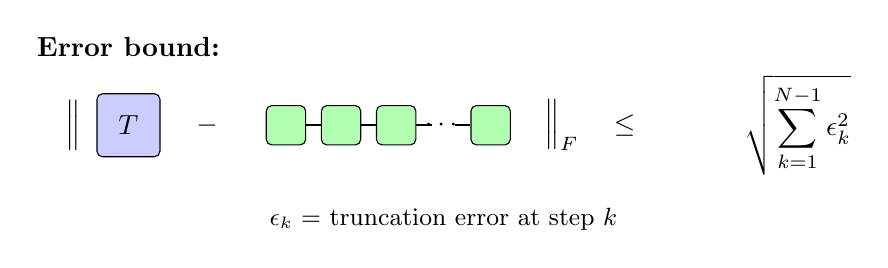
\begin{tikzpicture}[scale=1]
    \node[font=\bfseries] at (0, 1) {Error bound:};

    % Original tensor
    \node[tensor] (T) at (0,0) {$T$};

    \node at (1,0) {$-$};

    % Approximate TT
    \node[tensorA, minimum size=0.5cm] (A1) at (2,0) {};
    \draw[bond] (A1.east) -- ++(0.2,0);
    \node[tensorA, minimum size=0.5cm] (A2) at (2.7,0) {};
    \draw[bond] (A2.east) -- ++(0.2,0);
    \node[tensorA, minimum size=0.5cm] (A3) at (3.4,0) {};
    \draw[bond] (A3.east) -- ++(0.2,0);
    \node at (4.0,0) {$\cdots$};
    \node[tensorA, minimum size=0.5cm] (AN) at (4.6,0) {};
    \draw[bond] (AN.west) -- ++(-0.2,0);

    % Frobenius norm
    \node at (5.5, 0) {$\Big\|_F$};
    \node at (-0.7, 0) {$\Big\|$};

    % Inequality
    \node at (6.3, 0) {$\leq$};

    % Error bound
    \node at (8.5, 0) {$\displaystyle\sqrt{\sum_{k=1}^{N-1} \epsilon_k^2}$};

    % Explanation
    \node[font=\small, align=left] at (4, -1.2) {$\epsilon_k$ = truncation error at step $k$};
\end{tikzpicture}

\end{document}
